\chapter{KMALL Stage}

Recent advances in sonar technology and computing power have led to an improvement in ocean monitoring. For instance, Multibeam Echosounders (MBES) are now capable of collecting data from the water column, besides some usual metrics as seafloor reflectivity. This new information allows geoscientists to identify sunken structures, schools of fish, gas seeps, etc.

\begin{figure}[h!]
	\begin{center}
		  \begin{tabular}{ @{} c @{} }
			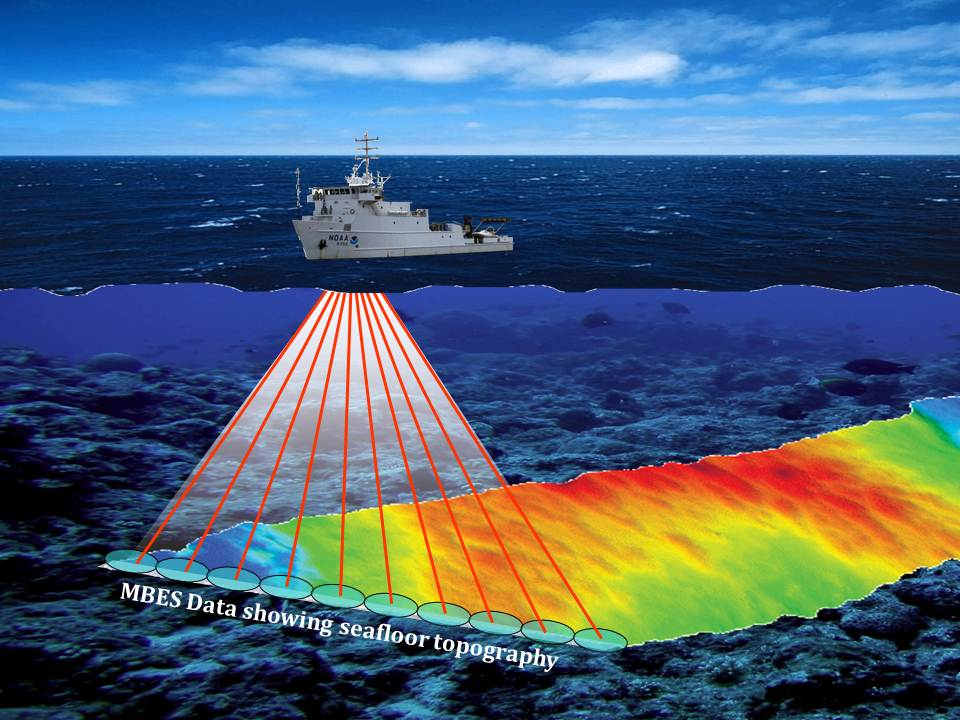
\includegraphics[scale=0.45]{images/mbes_ship.jpg}\\
			\imagesource{NOAA Photo Library, CC BY 2.0, via Wikimedia Commons.}
		\end{tabular}
	\end{center}
	\vspace*{-0.7em}
	\caption{Conception of multibeam sonar on NOAA Ship NANCY FOSTER.}
	\label{fig:mbes_ship}
\end{figure}

We clearly see that water column metrics have a big interest. However, their storage requirements are quite demanding (in the order of some GB/h). Hence, although it is possible to continuously record water column data, in practice it is only used in some specific explorations such as gas-seeps zones. In this scenario, efficient compression algorithms will be essential.

At the present moment, one of the biggest echosounder manufacturers is Kongsberg Maritime, a company with more than 7000 employees over 25 countries. In this chapter we will focus on the development of a preprocessing stage specially designed for the KMALL files from Kongsberg. First, a general overview of the data structures will be given. Then, with this format in mind, a design criterion will be proposed and implemented. Finally, we will analyze its performance and compare it with other compression algorithms.

\section{The KMALL data format}
In this section we will describe the KMALL data structure and why there is a need to develop new compression algorithms for this format, but first some concepts related to echosounders must be defined:
\begin{itemize}
	\item \textbf{Ping:} A ping is defined as a number of pulses transmitted at approximately the same time.
	\item \textbf{Beam:} Each ping is formed by some pulses in different angles, which we call beams.
\end{itemize}

Notice that the number of beams per ping depends on each sonar model, and the numbers of samples per beam depends on the angle and on the depth. This dependence can be seen in figure \ref{fig:wc_data}.

The .kmall format is a new format from Kongsberg which has just started being implemented in new echosounder models. It is the successor of the Kongsberg .all format. Analyzing the latter is out of the scope of this project, yet we can state some of the improvements that KMALL brings.

On the first hand, KMALL is a generic format with high resolution data and with a datagram structure designed to avoid breaking existing decoders when updating the data structure.

On the other hand, .all format used to have a datagram size constraint of 64 kB due to the maximum size of UDP packets, but .kmall files are designed to be stored "as is" and then fragmented if needed. Its main advantage is that pings are not splitted between datagrams.

The size of a .kmall file is not fixed. Actually, the echosounder operator decides when the file being recorded at that moment should end. In our dataset, most of the files are between 100 and 400 MB. Inside these files there are several datagrams, which will be described later in this section.

The mixture of data types in the same file makes it difficult for standard compressors like \textit{Zip} to identify data statistics, therefore they don't perform as good as one could expect. In order to improve the compression ratio, we are interested in knowing how are those datagrams placed inside the file and how to identify them. From Kongsberg KMALL documentation, we know that all datagrams start with a generic header that contains datagram size in bytes and a 4-character identifier. In the current version (410224 Revision H), there exist the following datagram types:

\begin{table}[h!]
\footnotesize
\begin{center}
\resizebox{\textwidth}{!}{
\begin{tabular}{|l|l|l|}
	\hline
	\rowcolor[HTML]{9698ED} 
	\multicolumn{1}{|c|}{\cellcolor[HTML]{9698ED}Type code} & \multicolumn{1}{c|}{\cellcolor[HTML]{9698ED}Struct name} & \multicolumn{1}{c|}{\cellcolor[HTML]{9698ED}Description} \\ \hline
	\#IIP                                                   & EMdgmIIP\_def                                            & Installation and sensor parameters.                      \\ \hline
	\#IOP                                                   & EMdgmIOP\_def                                            & Runtime operator parameters.                             \\ \hline
	\#IBE                                                   & EMdgmIB\_def                                             & Built in test (BIST) error report.                       \\ \hline
	\#IBR                                                   & EMdgmIB\_def                                             & Built in test (BIST) reply.                              \\ \hline
	\#IBS                                                   & EMdgmIB\_def                                             & Built in test (BIST) short reply.                        \\ \hline
\end{tabular}}
\end{center}
\caption{Installation and runtime datagrams of the KMALL format.}
\end{table}

\begin{table}[h!]
\footnotesize
\begin{center}
\resizebox{\textwidth}{!}{
\begin{tabular}{|l|l|l|}
	\hline
	\rowcolor[HTML]{9698ED} 
	\multicolumn{1}{|c|}{\cellcolor[HTML]{9698ED}Type code} & \multicolumn{1}{c|}{\cellcolor[HTML]{9698ED}Struct name} & \multicolumn{1}{c|}{\cellcolor[HTML]{9698ED}Description}                                              \\ \hline
	\#SPO                                                   & EMdgmSPO\_def                                            & Sensor (S) data for position (PO).                                                                    \\ \hline
	\#SKM                                                   & EMdgmSKM\_def                                            & Sensor (S) KM binary sensor format.                                                                   \\ \hline
	\#SVP                                                   & EMdgmSVP\_def                                            & \begin{tabular}[c]{@{}l@{}}Sensor (S) data from sound velocity (V)\\ profile (P) or CTD.\end{tabular} \\ \hline
	\#SVT                                                   & EMdgmSVT\_def                                            & \begin{tabular}[c]{@{}l@{}}Sensor (S) data for sound velocity (V)\\ at transducer (T).\end{tabular}   \\ \hline
	\#SCL                                                   & EMdgmSCL\_def                                            & Sensor (S) data from clock (CL).                                                                      \\ \hline
	\#SDE                                                   & EMdgmSDE\_def                                            & Sensor (S) data from depth (DE) sensor.                                                               \\ \hline
	\#SHI                                                   & EMdgmSHI\_def                                            & Sensor (S) data for height (HI).                                                                      \\ \hline
\end{tabular}}
\end{center}
\caption{External sensor output datagrams of the KMALL format.}
\end{table}

\begin{table}[H]
\footnotesize
\begin{center}
\resizebox{\textwidth}{!}{
\begin{tabular}{|l|l|l|}
	\hline
	\rowcolor[HTML]{9698ED} 
	\multicolumn{1}{|c|}{\cellcolor[HTML]{9698ED}Type code} & \multicolumn{1}{c|}{\cellcolor[HTML]{9698ED}Struct name} & \multicolumn{1}{c|}{\cellcolor[HTML]{9698ED}Description} \\ \hline
	\#CPO                                                   & EMdgmCPO\_def                                            & Compatibility (C) data for position (PO).                \\ \hline
	\#CHE                                                   & EMdgmCHE\_def                                            & Compatibility (C) data for heave (HE).                   \\ \hline
\end{tabular}}
\end{center}
\caption{Compatibility datagrams of the KMALL format.}
\end{table}

\begin{table}[H]
\footnotesize
\begin{center}
\resizebox{\textwidth}{!}{
\begin{tabular}{|l|l|l|}
	\hline
	\rowcolor[HTML]{9698ED}
	\multicolumn{1}{|c|}{\cellcolor[HTML]{9698ED}Type code} & \multicolumn{1}{c|}{\cellcolor[HTML]{9698ED}Struct name} & \multicolumn{1}{c|}{\cellcolor[HTML]{9698ED}Description} \\ \hline
	\#FCF                                                   & EMdgmFCF\_def                                            & Backscatter calibration (C) file (F) datagram.           \\ \hline
\end{tabular}}
\end{center}
\caption{File datagrams of the KMALL format.}
\end{table}

\begin{table}[h!]
\footnotesize
\begin{center}
\resizebox{\textwidth}{!}{
	\begin{tabular}{|l|l|l|}
		\hline
		\rowcolor[HTML]{9698ED} 
		\multicolumn{1}{|c|}{\cellcolor[HTML]{9698ED}Type code} & \multicolumn{1}{c|}{\cellcolor[HTML]{9698ED}Struct name} & \multicolumn{1}{c|}{\cellcolor[HTML]{9698ED}Description}                                      \\ \hline
		\#MRZ                                                   & EMdgmMRZ\_def                                            & \begin{tabular}[c]{@{}l@{}}Multibeam (M) raw range (R)\\ and depth (Z) datagram.\end{tabular} \\ \hline
		\#MWC                                                   & EMdgmMWC\_def                                            & \begin{tabular}[c]{@{}l@{}}Multibeam (M) water (W)\\ column (C) datagram.\end{tabular}        \\ \hline
\end{tabular}}
\end{center}
\caption{Multibeam datagrams of the KMALL format.}
\end{table}

It is important to notice that even though .kmall files can contain all the above datagrams, usually water column data is logged in a separate file with extension .kmwcd, as this kind of echosounders are not used to analyze the water column but for bathymetry. In other words, MWC datagrams will be placed in .kmwcd files instead of .kmall files, but the decoding process is the same for both extensions.

As we will see in the next section, we are specially interested in \acrshort{mwc} datagrams. Therefore, before continuing, we will describe them properly.

\subsection{\acrshort{mwc} datagrams}

\acrshort{mwc} datagrams are structured as follows:

\begin{figure}[h!]
	\begin{center}
		\scalebox{.565}{% Graphic for TeX using PGF
% Title: /home/aniol/Documents/Uni/Telecos/TFG/mwc_datagram.dia
% Creator: Dia v0.97+git
% CreationDate: Fri Feb 12 18:10:30 2021
% For: aniol
% \usepackage{tikz}
% The following commands are not supported in PSTricks at present
% We define them conditionally, so when they are implemented,
% this pgf file will use them.
\ifx\du\undefined
  \newlength{\du}
\fi
\setlength{\du}{15\unitlength}
\begin{tikzpicture}[even odd rule]
\pgftransformxscale{1.000000}
\pgftransformyscale{-1.000000}
\definecolor{dialinecolor}{rgb}{0.000000, 0.000000, 0.000000}
\pgfsetstrokecolor{dialinecolor}
\pgfsetstrokeopacity{1.000000}
\definecolor{diafillcolor}{rgb}{1.000000, 1.000000, 1.000000}
\pgfsetfillcolor{diafillcolor}
\pgfsetfillopacity{1.000000}
\pgfsetlinewidth{0.100000\du}
\pgfsetdash{}{0pt}
\pgfsetmiterjoin
\pgfsetbuttcap
{\pgfsetcornersarced{\pgfpoint{0.000000\du}{0.000000\du}}\definecolor{diafillcolor}{rgb}{1.000000, 1.000000, 1.000000}
\pgfsetfillcolor{diafillcolor}
\pgfsetfillopacity{1.000000}
\fill (2.100000\du,9.900000\du)--(2.100000\du,15.000000\du)--(52.000000\du,15.000000\du)--(52.000000\du,9.900000\du)--cycle;
}{\pgfsetcornersarced{\pgfpoint{0.000000\du}{0.000000\du}}\definecolor{dialinecolor}{rgb}{0.000000, 0.000000, 0.000000}
\pgfsetstrokecolor{dialinecolor}
\pgfsetstrokeopacity{1.000000}
\draw (2.100000\du,9.900000\du)--(2.100000\du,15.000000\du)--(52.000000\du,15.000000\du)--(52.000000\du,9.900000\du)--cycle;
}\pgfsetlinewidth{0.100000\du}
\pgfsetdash{}{0pt}
\pgfsetbuttcap
{
\definecolor{diafillcolor}{rgb}{0.000000, 0.000000, 0.000000}
\pgfsetfillcolor{diafillcolor}
\pgfsetfillopacity{1.000000}
% was here!!!
\definecolor{dialinecolor}{rgb}{0.000000, 0.000000, 0.000000}
\pgfsetstrokecolor{dialinecolor}
\pgfsetstrokeopacity{1.000000}
\draw (7.058330\du,9.850000\du)--(7.058330\du,15.031300\du);
}
% setfont left to latex
\definecolor{dialinecolor}{rgb}{0.000000, 0.000000, 0.000000}
\pgfsetstrokecolor{dialinecolor}
\pgfsetstrokeopacity{1.000000}
\definecolor{diafillcolor}{rgb}{0.000000, 0.000000, 0.000000}
\pgfsetfillcolor{diafillcolor}
\pgfsetfillopacity{1.000000}
\node[anchor=base,inner sep=0pt, outer sep=0pt,color=dialinecolor] at (4.516770\du,12.193700\du){Header};
% setfont left to latex
\definecolor{dialinecolor}{rgb}{0.000000, 0.000000, 0.000000}
\pgfsetstrokecolor{dialinecolor}
\pgfsetstrokeopacity{1.000000}
\definecolor{diafillcolor}{rgb}{0.000000, 0.000000, 0.000000}
\pgfsetfillcolor{diafillcolor}
\pgfsetfillopacity{1.000000}
\node[anchor=base,inner sep=0pt, outer sep=0pt,color=dialinecolor] at (4.516770\du,12.993700\du){20 \ensuremath{[}B\ensuremath{]}};
\pgfsetlinewidth{0.100000\du}
\pgfsetdash{}{0pt}
\pgfsetbuttcap
{
\definecolor{diafillcolor}{rgb}{0.000000, 0.000000, 0.000000}
\pgfsetfillcolor{diafillcolor}
\pgfsetfillopacity{1.000000}
% was here!!!
\definecolor{dialinecolor}{rgb}{0.000000, 0.000000, 0.000000}
\pgfsetstrokecolor{dialinecolor}
\pgfsetstrokeopacity{1.000000}
\draw (10.606800\du,9.867080\du)--(10.606800\du,15.048300\du);
}
% setfont left to latex
\definecolor{dialinecolor}{rgb}{0.000000, 0.000000, 0.000000}
\pgfsetstrokecolor{dialinecolor}
\pgfsetstrokeopacity{1.000000}
\definecolor{diafillcolor}{rgb}{0.000000, 0.000000, 0.000000}
\pgfsetfillcolor{diafillcolor}
\pgfsetfillopacity{1.000000}
\node[anchor=base,inner sep=0pt, outer sep=0pt,color=dialinecolor] at (8.850100\du,12.193800\du){Partition};
% setfont left to latex
\definecolor{dialinecolor}{rgb}{0.000000, 0.000000, 0.000000}
\pgfsetstrokecolor{dialinecolor}
\pgfsetstrokeopacity{1.000000}
\definecolor{diafillcolor}{rgb}{0.000000, 0.000000, 0.000000}
\pgfsetfillcolor{diafillcolor}
\pgfsetfillopacity{1.000000}
\node[anchor=base,inner sep=0pt, outer sep=0pt,color=dialinecolor] at (8.850100\du,12.993800\du){4 \ensuremath{[}B\ensuremath{]}};
\pgfsetlinewidth{0.100000\du}
\pgfsetdash{}{0pt}
\pgfsetbuttcap
{
\definecolor{diafillcolor}{rgb}{0.000000, 0.000000, 0.000000}
\pgfsetfillcolor{diafillcolor}
\pgfsetfillopacity{1.000000}
% was here!!!
\definecolor{dialinecolor}{rgb}{0.000000, 0.000000, 0.000000}
\pgfsetstrokecolor{dialinecolor}
\pgfsetstrokeopacity{1.000000}
\draw (15.140100\du,9.867080\du)--(15.140100\du,15.048300\du);
}
% setfont left to latex
\definecolor{dialinecolor}{rgb}{0.000000, 0.000000, 0.000000}
\pgfsetstrokecolor{dialinecolor}
\pgfsetstrokeopacity{1.000000}
\definecolor{diafillcolor}{rgb}{0.000000, 0.000000, 0.000000}
\pgfsetfillcolor{diafillcolor}
\pgfsetfillopacity{1.000000}
\node[anchor=base,inner sep=0pt, outer sep=0pt,color=dialinecolor] at (12.883400\du,12.193800\du){CmnPart};
% setfont left to latex
\definecolor{dialinecolor}{rgb}{0.000000, 0.000000, 0.000000}
\pgfsetstrokecolor{dialinecolor}
\pgfsetstrokeopacity{1.000000}
\definecolor{diafillcolor}{rgb}{0.000000, 0.000000, 0.000000}
\pgfsetfillcolor{diafillcolor}
\pgfsetfillopacity{1.000000}
\node[anchor=base,inner sep=0pt, outer sep=0pt,color=dialinecolor] at (12.883400\du,12.993800\du){12 \ensuremath{[}B\ensuremath{]}};
\pgfsetlinewidth{0.100000\du}
\pgfsetdash{}{0pt}
\pgfsetbuttcap
{
\definecolor{diafillcolor}{rgb}{0.000000, 0.000000, 0.000000}
\pgfsetfillcolor{diafillcolor}
\pgfsetfillopacity{1.000000}
% was here!!!
\definecolor{dialinecolor}{rgb}{0.000000, 0.000000, 0.000000}
\pgfsetstrokecolor{dialinecolor}
\pgfsetstrokeopacity{1.000000}
\draw (19.780100\du,9.857080\du)--(19.780100\du,15.038300\du);
}
% setfont left to latex
\definecolor{dialinecolor}{rgb}{0.000000, 0.000000, 0.000000}
\pgfsetstrokecolor{dialinecolor}
\pgfsetstrokeopacity{1.000000}
\definecolor{diafillcolor}{rgb}{0.000000, 0.000000, 0.000000}
\pgfsetfillcolor{diafillcolor}
\pgfsetfillopacity{1.000000}
\node[anchor=base,inner sep=0pt, outer sep=0pt,color=dialinecolor] at (17.483400\du,12.193700\du){TxInfo};
% setfont left to latex
\definecolor{dialinecolor}{rgb}{0.000000, 0.000000, 0.000000}
\pgfsetstrokecolor{dialinecolor}
\pgfsetstrokeopacity{1.000000}
\definecolor{diafillcolor}{rgb}{0.000000, 0.000000, 0.000000}
\pgfsetfillcolor{diafillcolor}
\pgfsetfillopacity{1.000000}
\node[anchor=base,inner sep=0pt, outer sep=0pt,color=dialinecolor] at (17.483400\du,12.993700\du){12 \ensuremath{[}B\ensuremath{]}};
\pgfsetlinewidth{0.100000\du}
\pgfsetdash{}{0pt}
\pgfsetbuttcap
{
\definecolor{diafillcolor}{rgb}{0.000000, 0.000000, 0.000000}
\pgfsetfillcolor{diafillcolor}
\pgfsetfillopacity{1.000000}
% was here!!!
\definecolor{dialinecolor}{rgb}{0.000000, 0.000000, 0.000000}
\pgfsetstrokecolor{dialinecolor}
\pgfsetstrokeopacity{1.000000}
\draw (27.206700\du,9.865000\du)--(27.206700\du,15.046200\du);
}
% setfont left to latex
\definecolor{dialinecolor}{rgb}{0.000000, 0.000000, 0.000000}
\pgfsetstrokecolor{dialinecolor}
\pgfsetstrokeopacity{1.000000}
\definecolor{diafillcolor}{rgb}{0.000000, 0.000000, 0.000000}
\pgfsetfillcolor{diafillcolor}
\pgfsetfillopacity{1.000000}
\node[anchor=base,inner sep=0pt, outer sep=0pt,color=dialinecolor] at (23.516700\du,12.158400\du){SectorData};
% setfont left to latex
\definecolor{dialinecolor}{rgb}{0.000000, 0.000000, 0.000000}
\pgfsetstrokecolor{dialinecolor}
\pgfsetstrokeopacity{1.000000}
\definecolor{diafillcolor}{rgb}{0.000000, 0.000000, 0.000000}
\pgfsetfillcolor{diafillcolor}
\pgfsetfillopacity{1.000000}
\node[anchor=base,inner sep=0pt, outer sep=0pt,color=dialinecolor] at (23.516700\du,12.958400\du){9 x 16 \ensuremath{[}B\ensuremath{]}};
\pgfsetlinewidth{0.100000\du}
\pgfsetdash{}{0pt}
\pgfsetbuttcap
{
\definecolor{diafillcolor}{rgb}{0.000000, 0.000000, 0.000000}
\pgfsetfillcolor{diafillcolor}
\pgfsetfillopacity{1.000000}
% was here!!!
\definecolor{dialinecolor}{rgb}{0.000000, 0.000000, 0.000000}
\pgfsetstrokecolor{dialinecolor}
\pgfsetstrokeopacity{1.000000}
\draw (32.580000\du,9.855000\du)--(32.580000\du,15.036200\du);
}
% setfont left to latex
\definecolor{dialinecolor}{rgb}{0.000000, 0.000000, 0.000000}
\pgfsetstrokecolor{dialinecolor}
\pgfsetstrokeopacity{1.000000}
\definecolor{diafillcolor}{rgb}{0.000000, 0.000000, 0.000000}
\pgfsetfillcolor{diafillcolor}
\pgfsetfillopacity{1.000000}
\node[anchor=base,inner sep=0pt, outer sep=0pt,color=dialinecolor] at (29.950000\du,12.158300\du){RxInfo};
% setfont left to latex
\definecolor{dialinecolor}{rgb}{0.000000, 0.000000, 0.000000}
\pgfsetstrokecolor{dialinecolor}
\pgfsetstrokeopacity{1.000000}
\definecolor{diafillcolor}{rgb}{0.000000, 0.000000, 0.000000}
\pgfsetfillcolor{diafillcolor}
\pgfsetfillopacity{1.000000}
\node[anchor=base,inner sep=0pt, outer sep=0pt,color=dialinecolor] at (29.950000\du,12.958300\du){16 \ensuremath{[}B\ensuremath{]}};
% setfont left to latex
\definecolor{dialinecolor}{rgb}{0.000000, 0.000000, 0.000000}
\pgfsetstrokecolor{dialinecolor}
\pgfsetstrokeopacity{1.000000}
\definecolor{diafillcolor}{rgb}{0.000000, 0.000000, 0.000000}
\pgfsetfillcolor{diafillcolor}
\pgfsetfillopacity{1.000000}
\node[anchor=base,inner sep=0pt, outer sep=0pt,color=dialinecolor] at (42.150000\du,12.125000\du){BeamData};
% setfont left to latex
\definecolor{dialinecolor}{rgb}{0.000000, 0.000000, 0.000000}
\pgfsetstrokecolor{dialinecolor}
\pgfsetstrokeopacity{1.000000}
\definecolor{diafillcolor}{rgb}{0.000000, 0.000000, 0.000000}
\pgfsetfillcolor{diafillcolor}
\pgfsetfillopacity{1.000000}
\node[anchor=base,inner sep=0pt, outer sep=0pt,color=dialinecolor] at (42.150000\du,12.925000\du){$N_B \cdot (16 + N_S \cdot (1 + phaseFlag))$ \ensuremath{[}B\ensuremath{]}};
\end{tikzpicture}
}
	\end{center}
	\caption{MWC datagram as described by Kongsberg (410224 Revision H).}
	\label{fig:mwc_datagram}
\end{figure}

Where:
\begin{description}
	\item $N_B \equiv$ Number of beams in ping. It is stored as a 16-bit integer in \textit{RxInfo}.
	\item $N_S \equiv$ Number of samples in beam. It is stored as a 16-bit integer in \textit{BeamData}.
	\item $phaseFlag \equiv$ Flag that indicates if there is phase information after amplitude samples. It may be 0 (no phase information), 1 (low resolution) or 2 (high resolution). It is stored as an 8-bit integer in \textit{RxInfo}.
\end{description}

\begin{comment}
Caldria comentar més els camps del datagrama o així està bé?
\end{comment}

\section{Design}
\begin{comment}
Potser hauria de fer subseccions? "Requirements", "Datagrams to compress", "Criteria", etc.
\end{comment}

In the previous section we introduced the KMALL data format. Namely, we saw that it is a mixture of different data types, so we have to decide which ones should be compressed and which algorithm will be applied.

In order to decide what to compress, we have first analyzed some .kmall and .kmwcd to determine the percentage of occupancy by datagram type. For the former files, we found that MRZ datagrams are a 92\% of the total size; and for the later, MWC datagrams are a 99\%. It is clear that these two data types are our objective; however, in this thesis we will ignore MRZ datagrams and we will just focus on MWC data. Actually, if we look at figure \ref{fig:mwc_datagram} we see that MWC headers are insignificant compared to its samples, therefore we will only compress payload information.

\begin{figure}[h!]
	\begin{center}
		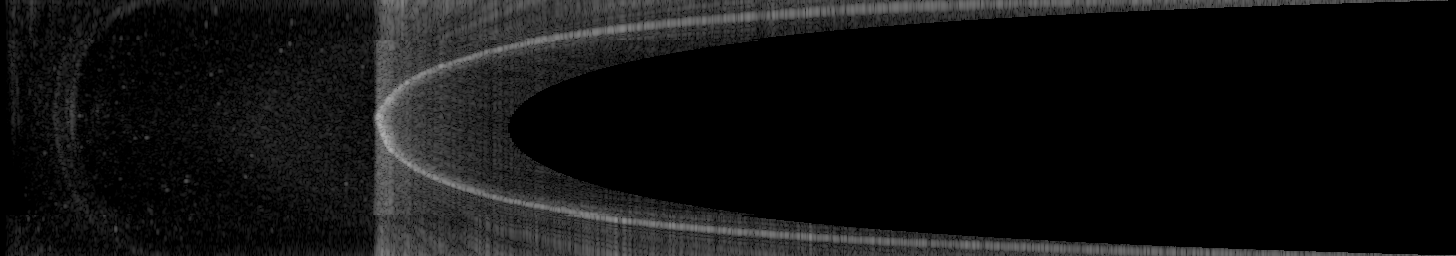
\includegraphics[scale=0.3]{images/water_column_data.png}
	\end{center}
	\caption{Raw image representation of the water column data captured by a Kongsberg EM 2040 echosounder.}
	\label{fig:wc_data}
\end{figure}


Once we have decided that we will restrict to water column data, a design criteria must be properly defined. This design has to take into account multiple aspects, namely: speed, implementation easiness and compression performance.

In previous chapters we explained that FAPEC compresses files by breaking them into chunks and processing each of them individually. This feature may be dangerous in our datagram scenario, so our first criterion will be to avoid FAPEC from splitting datagrams into different chunks. This way, the implementation will be much easier at the cost of reducing the process performance.

\begin{comment}
Estic anant massa per feina i sent poc curós, així que afegeixo la resta de criteris com a comentari i ja ho redactaré un altre dia.

Degut a l'estructura "parabòlica" de les mostres (pendent generar figura), cal vigilar en com les processem. La proposta és: per la secció quadrada restem respecte beam anterior (molt semblants). Per la secció parabòlica comprovem la diferència de mostres amb l'anterior i amb el simètric. Les opcions d'això són:

difAnt = 0, difSim = 0 => Ant\\
difAnt != 0, difSim != 0 => Ant\\
difAnt != 0, difSim = 0 => Sim

El motiu d'això és que està més correlat amb l'anterior i també cal més padding (el nombre de mostres entre beams decreix quadràticament), cosa bona per FAPEC (millor afegir 10 zeros que 2).
\end{comment}

\section{Implementation}
\begin{comment}
Implementació amb C de l'algoritme. El codi anirà als annexes (a poder ser confidencials).
\end{comment}

\section{Results}
\begin{comment}
No ens precipitem.
\end{comment}